% Options for packages loaded elsewhere
\PassOptionsToPackage{unicode}{hyperref}
\PassOptionsToPackage{hyphens}{url}
%
\documentclass[
  man,floatsintext]{apa7}
\usepackage{amsmath,amssymb}
\usepackage{lmodern}
\usepackage{iftex}
\ifPDFTeX
  \usepackage[T1]{fontenc}
  \usepackage[utf8]{inputenc}
  \usepackage{textcomp} % provide euro and other symbols
\else % if luatex or xetex
  \usepackage{unicode-math}
  \defaultfontfeatures{Scale=MatchLowercase}
  \defaultfontfeatures[\rmfamily]{Ligatures=TeX,Scale=1}
\fi
% Use upquote if available, for straight quotes in verbatim environments
\IfFileExists{upquote.sty}{\usepackage{upquote}}{}
\IfFileExists{microtype.sty}{% use microtype if available
  \usepackage[]{microtype}
  \UseMicrotypeSet[protrusion]{basicmath} % disable protrusion for tt fonts
}{}
\makeatletter
\@ifundefined{KOMAClassName}{% if non-KOMA class
  \IfFileExists{parskip.sty}{%
    \usepackage{parskip}
  }{% else
    \setlength{\parindent}{0pt}
    \setlength{\parskip}{6pt plus 2pt minus 1pt}}
}{% if KOMA class
  \KOMAoptions{parskip=half}}
\makeatother
\usepackage{xcolor}
\usepackage{graphicx}
\makeatletter
\def\maxwidth{\ifdim\Gin@nat@width>\linewidth\linewidth\else\Gin@nat@width\fi}
\def\maxheight{\ifdim\Gin@nat@height>\textheight\textheight\else\Gin@nat@height\fi}
\makeatother
% Scale images if necessary, so that they will not overflow the page
% margins by default, and it is still possible to overwrite the defaults
% using explicit options in \includegraphics[width, height, ...]{}
\setkeys{Gin}{width=\maxwidth,height=\maxheight,keepaspectratio}
% Set default figure placement to htbp
\makeatletter
\def\fps@figure{htbp}
\makeatother
\setlength{\emergencystretch}{3em} % prevent overfull lines
\providecommand{\tightlist}{%
  \setlength{\itemsep}{0pt}\setlength{\parskip}{0pt}}
\setcounter{secnumdepth}{-\maxdimen} % remove section numbering
% Make \paragraph and \subparagraph free-standing
\ifx\paragraph\undefined\else
  \let\oldparagraph\paragraph
  \renewcommand{\paragraph}[1]{\oldparagraph{#1}\mbox{}}
\fi
\ifx\subparagraph\undefined\else
  \let\oldsubparagraph\subparagraph
  \renewcommand{\subparagraph}[1]{\oldsubparagraph{#1}\mbox{}}
\fi
\newlength{\cslhangindent}
\setlength{\cslhangindent}{1.5em}
\newlength{\csllabelwidth}
\setlength{\csllabelwidth}{3em}
\newlength{\cslentryspacingunit} % times entry-spacing
\setlength{\cslentryspacingunit}{\parskip}
\newenvironment{CSLReferences}[2] % #1 hanging-ident, #2 entry spacing
 {% don't indent paragraphs
  \setlength{\parindent}{0pt}
  % turn on hanging indent if param 1 is 1
  \ifodd #1
  \let\oldpar\par
  \def\par{\hangindent=\cslhangindent\oldpar}
  \fi
  % set entry spacing
  \setlength{\parskip}{#2\cslentryspacingunit}
 }%
 {}
\usepackage{calc}
\newcommand{\CSLBlock}[1]{#1\hfill\break}
\newcommand{\CSLLeftMargin}[1]{\parbox[t]{\csllabelwidth}{#1}}
\newcommand{\CSLRightInline}[1]{\parbox[t]{\linewidth - \csllabelwidth}{#1}\break}
\newcommand{\CSLIndent}[1]{\hspace{\cslhangindent}#1}
\ifLuaTeX
\usepackage[bidi=basic]{babel}
\else
\usepackage[bidi=default]{babel}
\fi
\babelprovide[main,import]{english}
% get rid of language-specific shorthands (see #6817):
\let\LanguageShortHands\languageshorthands
\def\languageshorthands#1{}
% Manuscript styling
\usepackage{upgreek}
\captionsetup{font=singlespacing,justification=justified}

% Table formatting
\usepackage{longtable}
\usepackage{lscape}
% \usepackage[counterclockwise]{rotating}   % Landscape page setup for large tables
\usepackage{multirow}		% Table styling
\usepackage{tabularx}		% Control Column width
\usepackage[flushleft]{threeparttable}	% Allows for three part tables with a specified notes section
\usepackage{threeparttablex}            % Lets threeparttable work with longtable

% Create new environments so endfloat can handle them
% \newenvironment{ltable}
%   {\begin{landscape}\centering\begin{threeparttable}}
%   {\end{threeparttable}\end{landscape}}
\newenvironment{lltable}{\begin{landscape}\centering\begin{ThreePartTable}}{\end{ThreePartTable}\end{landscape}}

% Enables adjusting longtable caption width to table width
% Solution found at http://golatex.de/longtable-mit-caption-so-breit-wie-die-tabelle-t15767.html
\makeatletter
\newcommand\LastLTentrywidth{1em}
\newlength\longtablewidth
\setlength{\longtablewidth}{1in}
\newcommand{\getlongtablewidth}{\begingroup \ifcsname LT@\roman{LT@tables}\endcsname \global\longtablewidth=0pt \renewcommand{\LT@entry}[2]{\global\advance\longtablewidth by ##2\relax\gdef\LastLTentrywidth{##2}}\@nameuse{LT@\roman{LT@tables}} \fi \endgroup}

% \setlength{\parindent}{0.5in}
% \setlength{\parskip}{0pt plus 0pt minus 0pt}

% Overwrite redefinition of paragraph and subparagraph by the default LaTeX template
% See https://github.com/crsh/papaja/issues/292
\makeatletter
\renewcommand{\paragraph}{\@startsection{paragraph}{4}{\parindent}%
  {0\baselineskip \@plus 0.2ex \@minus 0.2ex}%
  {-1em}%
  {\normalfont\normalsize\bfseries\itshape\typesectitle}}

\renewcommand{\subparagraph}[1]{\@startsection{subparagraph}{5}{1em}%
  {0\baselineskip \@plus 0.2ex \@minus 0.2ex}%
  {-\z@\relax}%
  {\normalfont\normalsize\itshape\hspace{\parindent}{#1}\textit{\addperi}}{\relax}}
\makeatother

% \usepackage{etoolbox}
\makeatletter
\patchcmd{\HyOrg@maketitle}
  {\section{\normalfont\normalsize\abstractname}}
  {\section*{\normalfont\normalsize\abstractname}}
  {}{\typeout{Failed to patch abstract.}}
\patchcmd{\HyOrg@maketitle}
  {\section{\protect\normalfont{\@title}}}
  {\section*{\protect\normalfont{\@title}}}
  {}{\typeout{Failed to patch title.}}
\makeatother

\usepackage{xpatch}
\makeatletter
\xapptocmd\appendix
  {\xapptocmd\section
    {\addcontentsline{toc}{section}{\appendixname\ifoneappendix\else~\theappendix\fi\\: #1}}
    {}{\InnerPatchFailed}%
  }
{}{\PatchFailed}
\keywords{bilingualism, word learning, children, code-mixing, language switching}
\usepackage{lineno}

\linenumbers
\usepackage{csquotes}
\usepackage{amsmath}
\usepackage[labelformat=empty]{caption}
\usepackage{caption}
\usepackage[extra]{tipa}
\renewcommand{\topfraction}{1}
\renewcommand{\bottomfraction}{1}
\renewcommand{\textfraction}{.1}
\renewcommand{\floatpagefraction}{1}
\setcounter{topnumber}{9}
\setcounter{bottomnumber}{9}
\setcounter{totalnumber}{20}
\setcounter{dbltopnumber}{9}
\makeatletter
\renewcommand{\paragraph}{\@startsection{paragraph}{4}{\parindent}%
  {0\baselineskip \@plus 0.2ex \@minus 0.2ex}%
  {-1em}%
  {\normalfont\normalsize\bfseries\typesectitle}}

\renewcommand{\subparagraph}[1]{\@startsection{subparagraph}{5}{1em}%
  {0\baselineskip \@plus 0.2ex \@minus 0.2ex}%
  {-\z@\relax}%
  {\normalfont\normalsize\bfseries\itshape\hspace{\parindent}{#1}\textit{\addperi}}{\relax}}
\makeatother

\ifLuaTeX
  \usepackage{selnolig}  % disable illegal ligatures
\fi
\IfFileExists{bookmark.sty}{\usepackage{bookmark}}{\usepackage{hyperref}}
\IfFileExists{xurl.sty}{\usepackage{xurl}}{} % add URL line breaks if available
\urlstyle{same} % disable monospaced font for URLs
\hypersetup{
  pdftitle={Patterns of language switching and bilingual children's word learning: An experiment across two communities},
  pdfauthor={Rachel Ka-Ying Tsui1, Jessica E. Kosie2, Laia Fibla1, Casey Lew-Williams2, \& Krista Byers-Heinlein1},
  pdflang={en-EN},
  pdfkeywords={bilingualism, word learning, children, code-mixing, language switching},
  hidelinks,
  pdfcreator={LaTeX via pandoc}}

\title{Patterns of language switching and bilingual children's word learning: An experiment across two communities}
\author{Rachel Ka-Ying Tsui\textsuperscript{1}, Jessica E. Kosie\textsuperscript{2}, Laia Fibla\textsuperscript{1}, Casey Lew-Williams\textsuperscript{2}, \& Krista Byers-Heinlein\textsuperscript{1}}
\date{}


\shorttitle{Tablet Switch}

\authornote{

Correspondence concerning this article should be addressed to Rachel Ka-Ying Tsui, Department of Psychology, 7141 Sherbrooke St.~West, Montreal, QC, Canada, H2T1V2. Rachel Ka-Ying Tsui is now at Laboratory for Language Development, RIKEN Center for Brain Science, 2-1 Hirosawa, Wako-shi, Saitama, Japan, 351-0198. Email: \href{mailto:rachelkytsui@gmail.com}{\nolinkurl{rachelkytsui@gmail.com}}. Experiment material, analysis scripts, data set, and supplemental materials are available at \url{https://osf.io/8vk3b/}.. E-mail: \href{mailto:rachelkytsui@gmail.com}{\nolinkurl{rachelkytsui@gmail.com}}

}

\affiliation{\vspace{0.5cm}\textsuperscript{1} Concordia University\\\textsuperscript{2} Princeton University}

\abstract{%
Language switching is common in bilingual environments, including those of many bilingual children. Some bilingual children hear rapid switching that involves immediate translation of words (an \emph{`immediate-translation'} pattern), while others hear their languages most often in long blocks of a single language (a \emph{`one-language-at-a-time'} pattern). Our two-site experimental study compared two groups of developing bilinguals from different communities, and investigated whether differences in the timing of language switching impose different demands on bilingual children' learning of novel nouns in their two languages: do children learn differently if they hear a translation immediately vs.~if they hear translations more separated in time? Using an at-home online tablet word learning task, data were collected asynchronously from 3- to 5-year-old bilinguals from French--English bilingual families in Montreal, Canada (N = 31) and Spanish--English bilingual families in New Jersey, USA (N = 22). Results showed that bilingual children in both communities readily learned new words, and their performance was similar across the \emph{immediate-translation} and \emph{one-language-at-a-time} conditions. Our findings highlight that different types of bilingual interactions can provide equal learning opportunities for bilingual children's vocabulary development.
}



\begin{document}
\maketitle

\captionsetup[table]{labelformat=empty}

Many children around the world grow up in bilingual environments. For example, 18-25\% of children in Canada (Schott et al., 2022) and more than 33\% of children in the United States (Migration Policy Institute, 2021) grow up learning two or more languages. Caregivers often have concerns about supporting bilingual development (Quirk et al., 2022), but lack resources and information to guide their decisions (Ahooja et al., 2022). One question caregivers face is how to introduce new words so that children learn them in both languages. Should they switch between languages to provide immediate translations, or use one language at a time? To help address this question, this study examined how 3- to 5-year-old bilinguals from two communities --- French--English learners in Montreal and Spanish--English learners in New Jersey --- acquire new words across both of their languages in different language switching contexts.

\hypertarget{caregivers-language-switching}{%
\subsection{Caregivers' language switching}\label{caregivers-language-switching}}

Bilingual speakers have the ability to switch between two languages in their conversations (Myers-Scotton, 2017; Poplack, 1980), including families raising bilingual children (Byers-Heinlein, 2013; Kremin et al., 2021a). For example, at snack time, a French--English bilingual caregiver may say ``One more? \emph{C'est le dernier.} {[}It's the last one.{]}'' (example from Kremin et al., 2021a). Over time, bilingual children may accumulate many exposures to switches between languages (De Houwer, 2007; Kosie et al., in preparation). All bilingual caregivers in one study switched languages at least once during a short free-play session with their children, although there were large individual differences in the amount of switching (Bail et al., 2005). Interestingly, caregivers' attitudes towards multilingualism may also contribute to how often they switch between languages during caregiver-child interactions. For example, caregivers raising bilingual children in Quebec, Canada may switch less between languages if they have a less positive attitude towards childhood multilingualism (Kircher et al., 2022). Yet, bilingual children would still likely be exposed to language switches across different social contexts in their daily lives (Kosie et al., in preparation). For example, even when caregivers do not switch languages when interacting directly with their children, it is very common for them to do so with other people in the presence of their children (Carbajal \& Peperkamp, 2020), which may be a common source of exposure to language switching for children.

A particularly common moment for caregivers to switch between their languages is when teaching bilingual children new words. Some bilingual caregivers provide an immediate translation to their bilingual children when introducing new words (i.e., an \emph{`immediate-translation'} strategy) (Bail et al., 2015; Kremin et al., 2021a); for example, a Spanish--English caregiver may say ``Do you see that dog? \emph{Un perro!}''. Other bilingual caregivers interact with their children in long bouts using a single language (i.e., a \emph{`one-language-at-a-time'} strategy); for example, a French--English caregiver may use only English when reading books together with their child but use French for the rest of their day so that their child would hear the word ``dog'' during storytime and hear \emph{``chien''} at other times. These two common styles of exposing bilingual children to words are also manifested in formats of bilingual children's books (Ahooja et al., 2022), in which texts from two languages may be separated or blocked or the two languages may be interwoven in the same text (Brouillard et al., 2022; Read et al., 2021; Thibeault \& Matheson. 2020). Some bilingual caregivers may use these bilingual books as a resource to support their child's bilingual word learning (Benitez et al., 2022).

The way that bilingual caregivers switch between languages when interacting with their children may also depend on the context of the bilingual community they belong to. Bilinguals in different communities have different language attitudes and practices and, as a result, may code-switch differently (Poplack, 1988; Gardner-Chloros et al., 2005; Lawson \& Sachdev, 2000). Previous research has shown that, when interacting with their children, Spanish--English bilingual caregivers in the United States switch languages more often than French--English bilingual caregivers in Montreal, Canada (Bail et al., 2015; Kremin et al., 2021a), although these studies used different approaches (i.e.~a structured play session versus a day-long at-home audio recording) to measure the frequency of switching. Nonetheless, the status of languages in society or the goals and values of different bilingual communities may impact language switching practices. For the case of Spanish--English bilinguals in the United States, Spanish is an immigrant heritage language that is often given minimal support in social structures (such as public education) and is often at risk of not being used by young learners (De Houwer, 2007). Frequent language switching between Spanish and English may therefore serve as a tool to better establish social identity in Spanish--English bilinguals and also maintain the use of their heritage language in an English-dominant society (Montes-Alcalá, 2000; Toribio, 2002). On the other hand, although use of both French and English is quite normalized in Montreal Canada, bilinguals may switch less often for the reason that it may be perceived as relatively less polite (Buoy \& Nicoladis, 2018). Given that different communities inevitably vary in typical patterns of language switching, bilingual children growing up in these communities may have different experiences with language switching when they are learning words across their two languages.

\hypertarget{language-switching-and-childrens-word-learning}{%
\subsection{Language switching and children's word learning}\label{language-switching-and-childrens-word-learning}}

Given its prevalence in speech directed to bilingual children, it is important to consider potential effects of language switching on language development. Early theories posited that switching between languages could confuse bilingual children (Grammont, 1902; Ronjat 1913; see Fennell \& Lew-Williams, 2017). While subsequent theorists de-emphasized concerns about language confusion, there is evidence that language mixing and switching may be challenging for infants' learning. For example, language switching leads to momentary processing costs, where some types of code-switched sentences may be more difficult to process than single-language sentences (Byers-Heinlein et al., 2017; Morini \& Newman, 2019; Potter et al., 2019). It has also been reported that bilingual children who hear frequent switching in their language input have smaller vocabularies (Byers-Heinlein, 2013; Carbajal \& Peperkamp, 2020).

Yet, other studies show that language switching might in fact support language learning. In one study, 18- to 24-month-old bilingual children whose caregivers often switched languages within sentences were found to have larger vocabulary sizes (Bail, 2015). In another study, bilingual children exposed to more frequent language mixing were also more successful in segmenting words in both languages (Orena \& Polka, 2019). Other studies reported no relationship between children's experiences hearing language mixing and their vocabulary development (Place \& Hoff, 2011). Moreover, language switching does not necessarily cause a processing cost. For example, in one study, bilingual children could similarly identify target nouns in single-language sentences and in sentences with several switched words (Kremin et al., 2021b). Finally, there is evidence from home language recordings that bilingual caregivers may code-switch in a way that aims to support their children's learning (Kremin et al., 2021a). Together, these results are supported by the general observation that bilingual children who have been exposed to frequent language switching do successfully learn their two languages (Bail et al., 2015; De Houwer, 2007).

\hypertarget{the-current-study}{%
\subsection{The current study}\label{the-current-study}}

The current study aimed to further our understanding of bilingual children's word learning in the context of language switches, with the ultimate goal of informing caregivers about how different bilingual strategies might affect language acquisition. Using an at-home word learning task implemented on touchscreen devices, we investigated whether differences in the timing of language switching impose different demands on bilingual children's learning of novel nouns in their two languages: do children learn differently if they hear a translation immediately vs.~if they hear translations more separated in time? We also examined whether children's learning ability in these conditions would vary across different bilingual communities by comparing learners from Spanish--English learners in New Jersey and French--English learners in Montreal.

\hypertarget{methods}{%
\section{Methods}\label{methods}}

Ethics approval was obtained from the Concordia University Human Research Ethics Board (Certification \#10000439) and the Princeton University Behavioral Research Ethics Board (Certification \#7117). Informed consent was obtained from caregivers prior to their children's participation in the study. Data collection started in July 2021 at both locations and concluded in October 2021 in Montreal, Canada and August 2022 in New Jersey, USA, and thus occurred during the COVID-19 pandemic. The experiment was preregistered and all materials and analysis are available at \url{https://osf.io/8vk3b/}.

\hypertarget{participants}{%
\subsection{Participants}\label{participants}}

A total of 53 bilingual children aged 3 to 5 years (29 girls) who were born full term and without any reported language problems participated in the study. Of those, 31 French--English bilingual children were tested in Montreal (Mean age = 4.09 years, \(SD\) = 0.59, range = 3.04 -- 5.05), and 22 Spanish--English bilingual children were tested in New Jersey (Mean age = 4.05 years, \(SD\) = 0.72, range = 3.03 -- 5.26)\footnote{We deviated from the number of participants indicated in our preregistration (i.e., 30 bilingual children per site), due to difficulty in recruiting Spanish--English bilingual children.}. The linguistic context differs across the two sites: In Montreal both English and French are spoken widely in society and education is available in both languages; by contrast in New Jersey English is the major community language and education is largely available in English. Across both sites, bilingual children were recruited through social media advertisements and participants databases maintained by the respective labs. Another 12 children were recruited but excluded in the final sample due to not completing the experiment (n = 1), low birth weight or born preterm under 37 weeks (n = 4), below the preregistered minimum age of 36 months (n = 1), technical issues including data not being saved by the program (n = 2), one case where a caregiver explicitly mentioned that a child tended to change the response and touch the other image if the first touch was not registered by the program (n = 1), and finally, not meeting the language criteria (n = 3; see below).

Children's language proficiency was assessed via an online modified version of the Language Experience and Proficiency Questionnaire (LEAP-Q; Marian et al., 2007). Caregivers rated their children's proficiency in English and French (in Montreal) or in English and Spanish (in New Jersey), relative to same-aged peers on a scale of 0 (no proficiency at all) to 10 (native proficiency). Proficiency data were available for 49 out of the 53 children in the final sample (data were missing from 1 French--English and 3 Spanish--English children): 14 children had equal comprehension proficiency in both languages (8 French--English, 6 Spanish--English); 17 children were more proficient in English comprehension than French/Spanish (12 French--English, 5 Spanish--English); and 18 children were more proficient in French/Spanish than in English (10 French--English, 8 Spanish--English); please see the supplemental materials for the descriptive statistics of the proficiency scores. There were no significant differences in proficiency across communities. Children were included in the final sample if they had at least 7/10 reported comprehension score in each of their languages or an accuracy of at least 5/6 familiar word trials in each language\footnote{Our preregistration stated that children should meet both of these two stringent proficiency criteria to be included. However, we deviated by including children who met either one of the criteria because applying the original criteria resulted in exclusion of a higher than anticipated number of children (22 exclusions under the preregistered criteria, 3 under the new criteria) with a resulting smaller sample size and decreased statistical power. The results with the subsample meeting the more stringent preregistered criteria were similar and are reported in the supplemental materials at OSF (\url{https://osf.io/8vk3b/}).}. Finally, the sample was generally from a mid-to-high socioeconomic status, which was comparable across the two populations: 71\% of the mothers in Montreal and 73\% of the mothers in New Jersey had completed a university degree or higher.

\hypertarget{stimuli}{%
\subsection{Stimuli}\label{stimuli}}

\begin{figure}[H]

{\centering 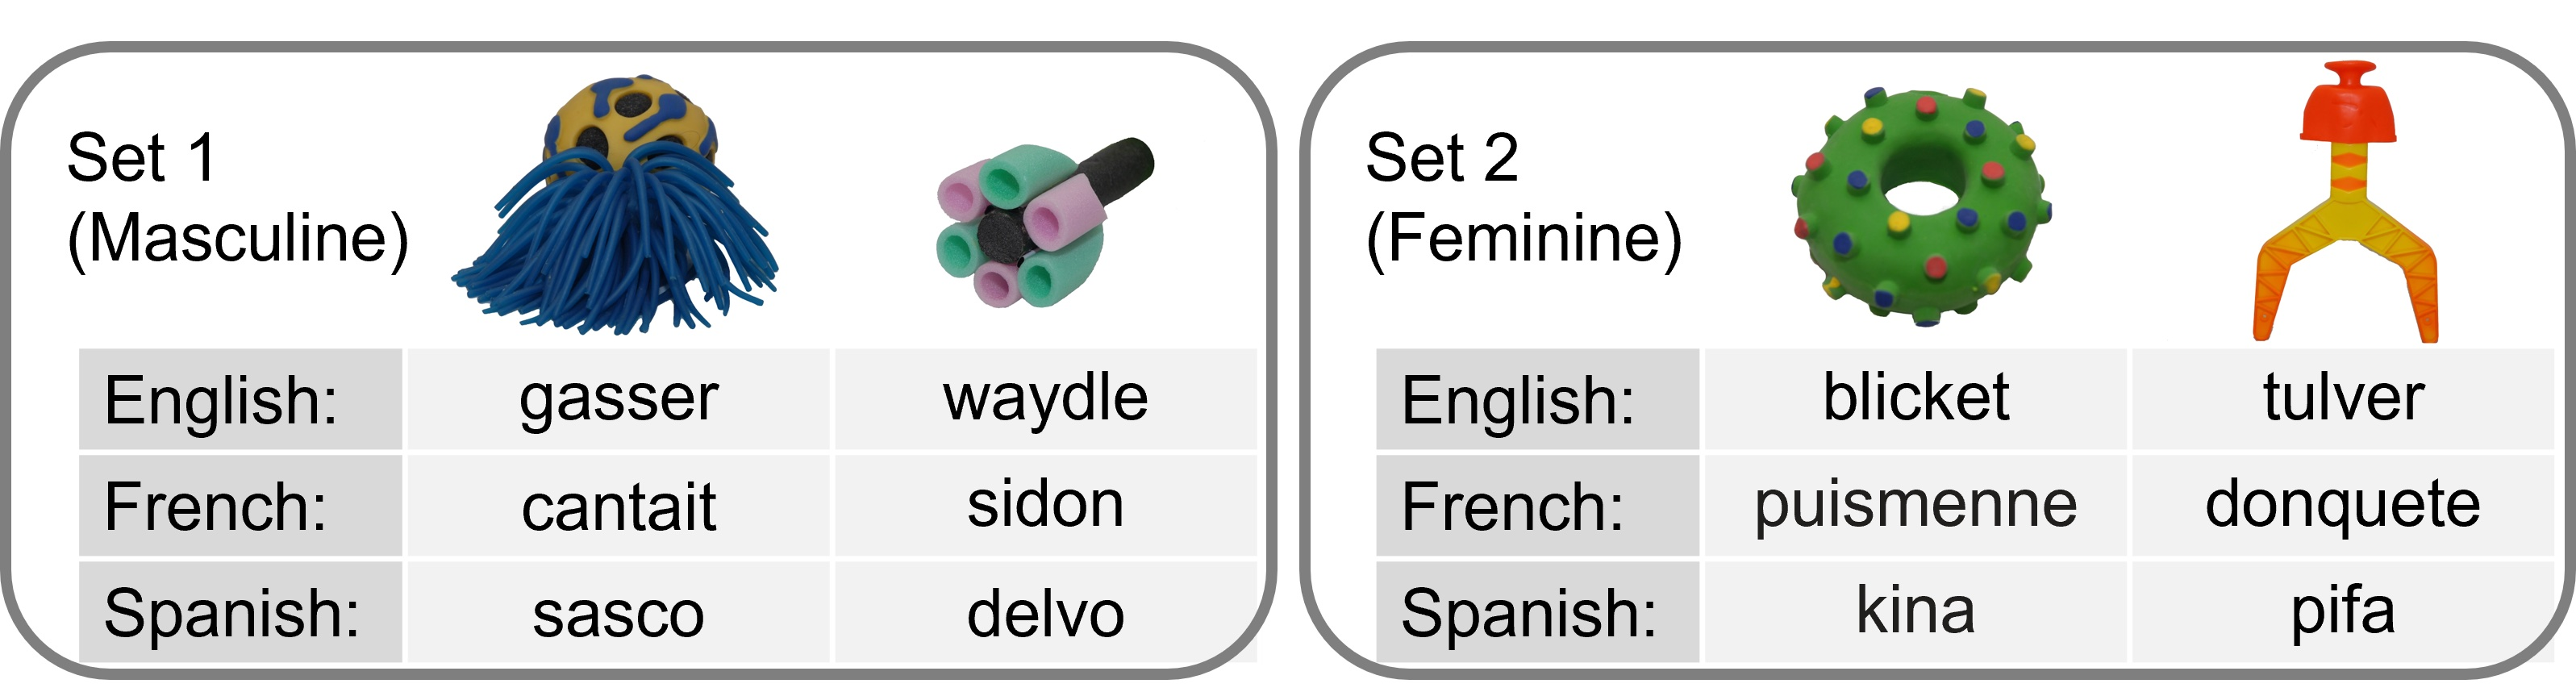
\includegraphics[width=0.8\linewidth]{/Users/racheltsui/Documents/GitHub/Bilingual-Families-Project_TabletSwitch/analysis/paper/figure/figure1} 

}

\caption{The four novel objects and their novel labels in English, French, and Spanish.}\label{fig:Figure1}
\end{figure}

Visual stimuli consisted of four distinct novel objects adapted from the Novel Object and Unusual Name (NOUN) Database (Horst \& Hout, 2016). Each object was given a unique, disyllabic novel label in English, French, and Spanish (see Figure 1 for the novel label-object pairings). Each label began with a distinct onset and was phonologically legal in its respective languages, and had a stress placement following the respective language's typical stress patterns (i.e., strong-weak stress in English and Spanish, and weak-strong stress in French).

The four novel label-object pairings were divided into two sets of two pairings, with Set 1 consisting of masculine-sounding French/Spanish labels and Set 2 of feminine-sounding French/Spanish labels, as judged by adult native speakers of each language. Set 1 was always presented in block 1 of the experiment and Set 2 in block 2. This design decision was made to avoid the possibility of not obtaining enough data for block 2 due to fatigue; however, all children did complete the experiment until the end of block 2, suggesting that the experiment was engaging to the children. With the experiment blocked by condition, which set a child saw in the two conditions depended on the block order which they were assigned to.

Auditory stimuli were recorded by a female native French--English or Spanish--English bilingual speaker using child-directed speech. Each of the four novel object labels were recorded in three different carrier phrases where the labels and the carrier phrases were always in the same language (e.g., ``Look, it's a \emph{blicket}. Touch it!'', ``Here's a \emph{blicket}. Touch it!'', and ``Touch the \emph{blicket}!''). Parallel sets were recorded in French (e.g., ``Regarde, c'est une \emph{puismenne}. Touche ça!'', ``Voici une \emph{puismenne}. Touche ça!'', and ``Touche la \emph{puismenne}!'')\footnote{For the French--English recording, the phrase ``Touch that''/\emph{``Touche ça''} was mistakenly recorded instead of ``Touch it''/\emph{``Touche el/la''}, but was retained as this difference was judged unlikely to affect children's performance.} and Spanish (e.g., ``Mira, es una \emph{kina}. Tócala!'', ``Aquí está una \emph{kina}. Tócala!'', and ``Toca la \emph{kina}!'').

\hypertarget{procedure}{%
\subsection{Procedure}\label{procedure}}

Children were tested at home asynchronously in an online tablet word-learning task. Prior to participation, caregivers gave written consent through email and were then asked to complete the LEAP-Q questionnaire rating their child's language proficiency. They were also given a link to the online tablet task, which was created using jsPsych (de Leeuw, 2015) and hosted on Pavlovia. Figure 2 illustrates the overall procedure (a sample video of the task is also available in our OSF site: \url{https://osf.io/8vk3b/}).

The task took up the full screen of the tablet and began with audio instructions provided to caregivers in their preferred language, which was unrelated to the language children would hear for the rest of the experiment. Caregivers were asked not to talk or give hints to their child, but should assist when technical difficulties occurred or repeat their child's touch when necessary (e.g., the child's touch was not properly registered by the device).

\begin{figure}[H]

{\centering 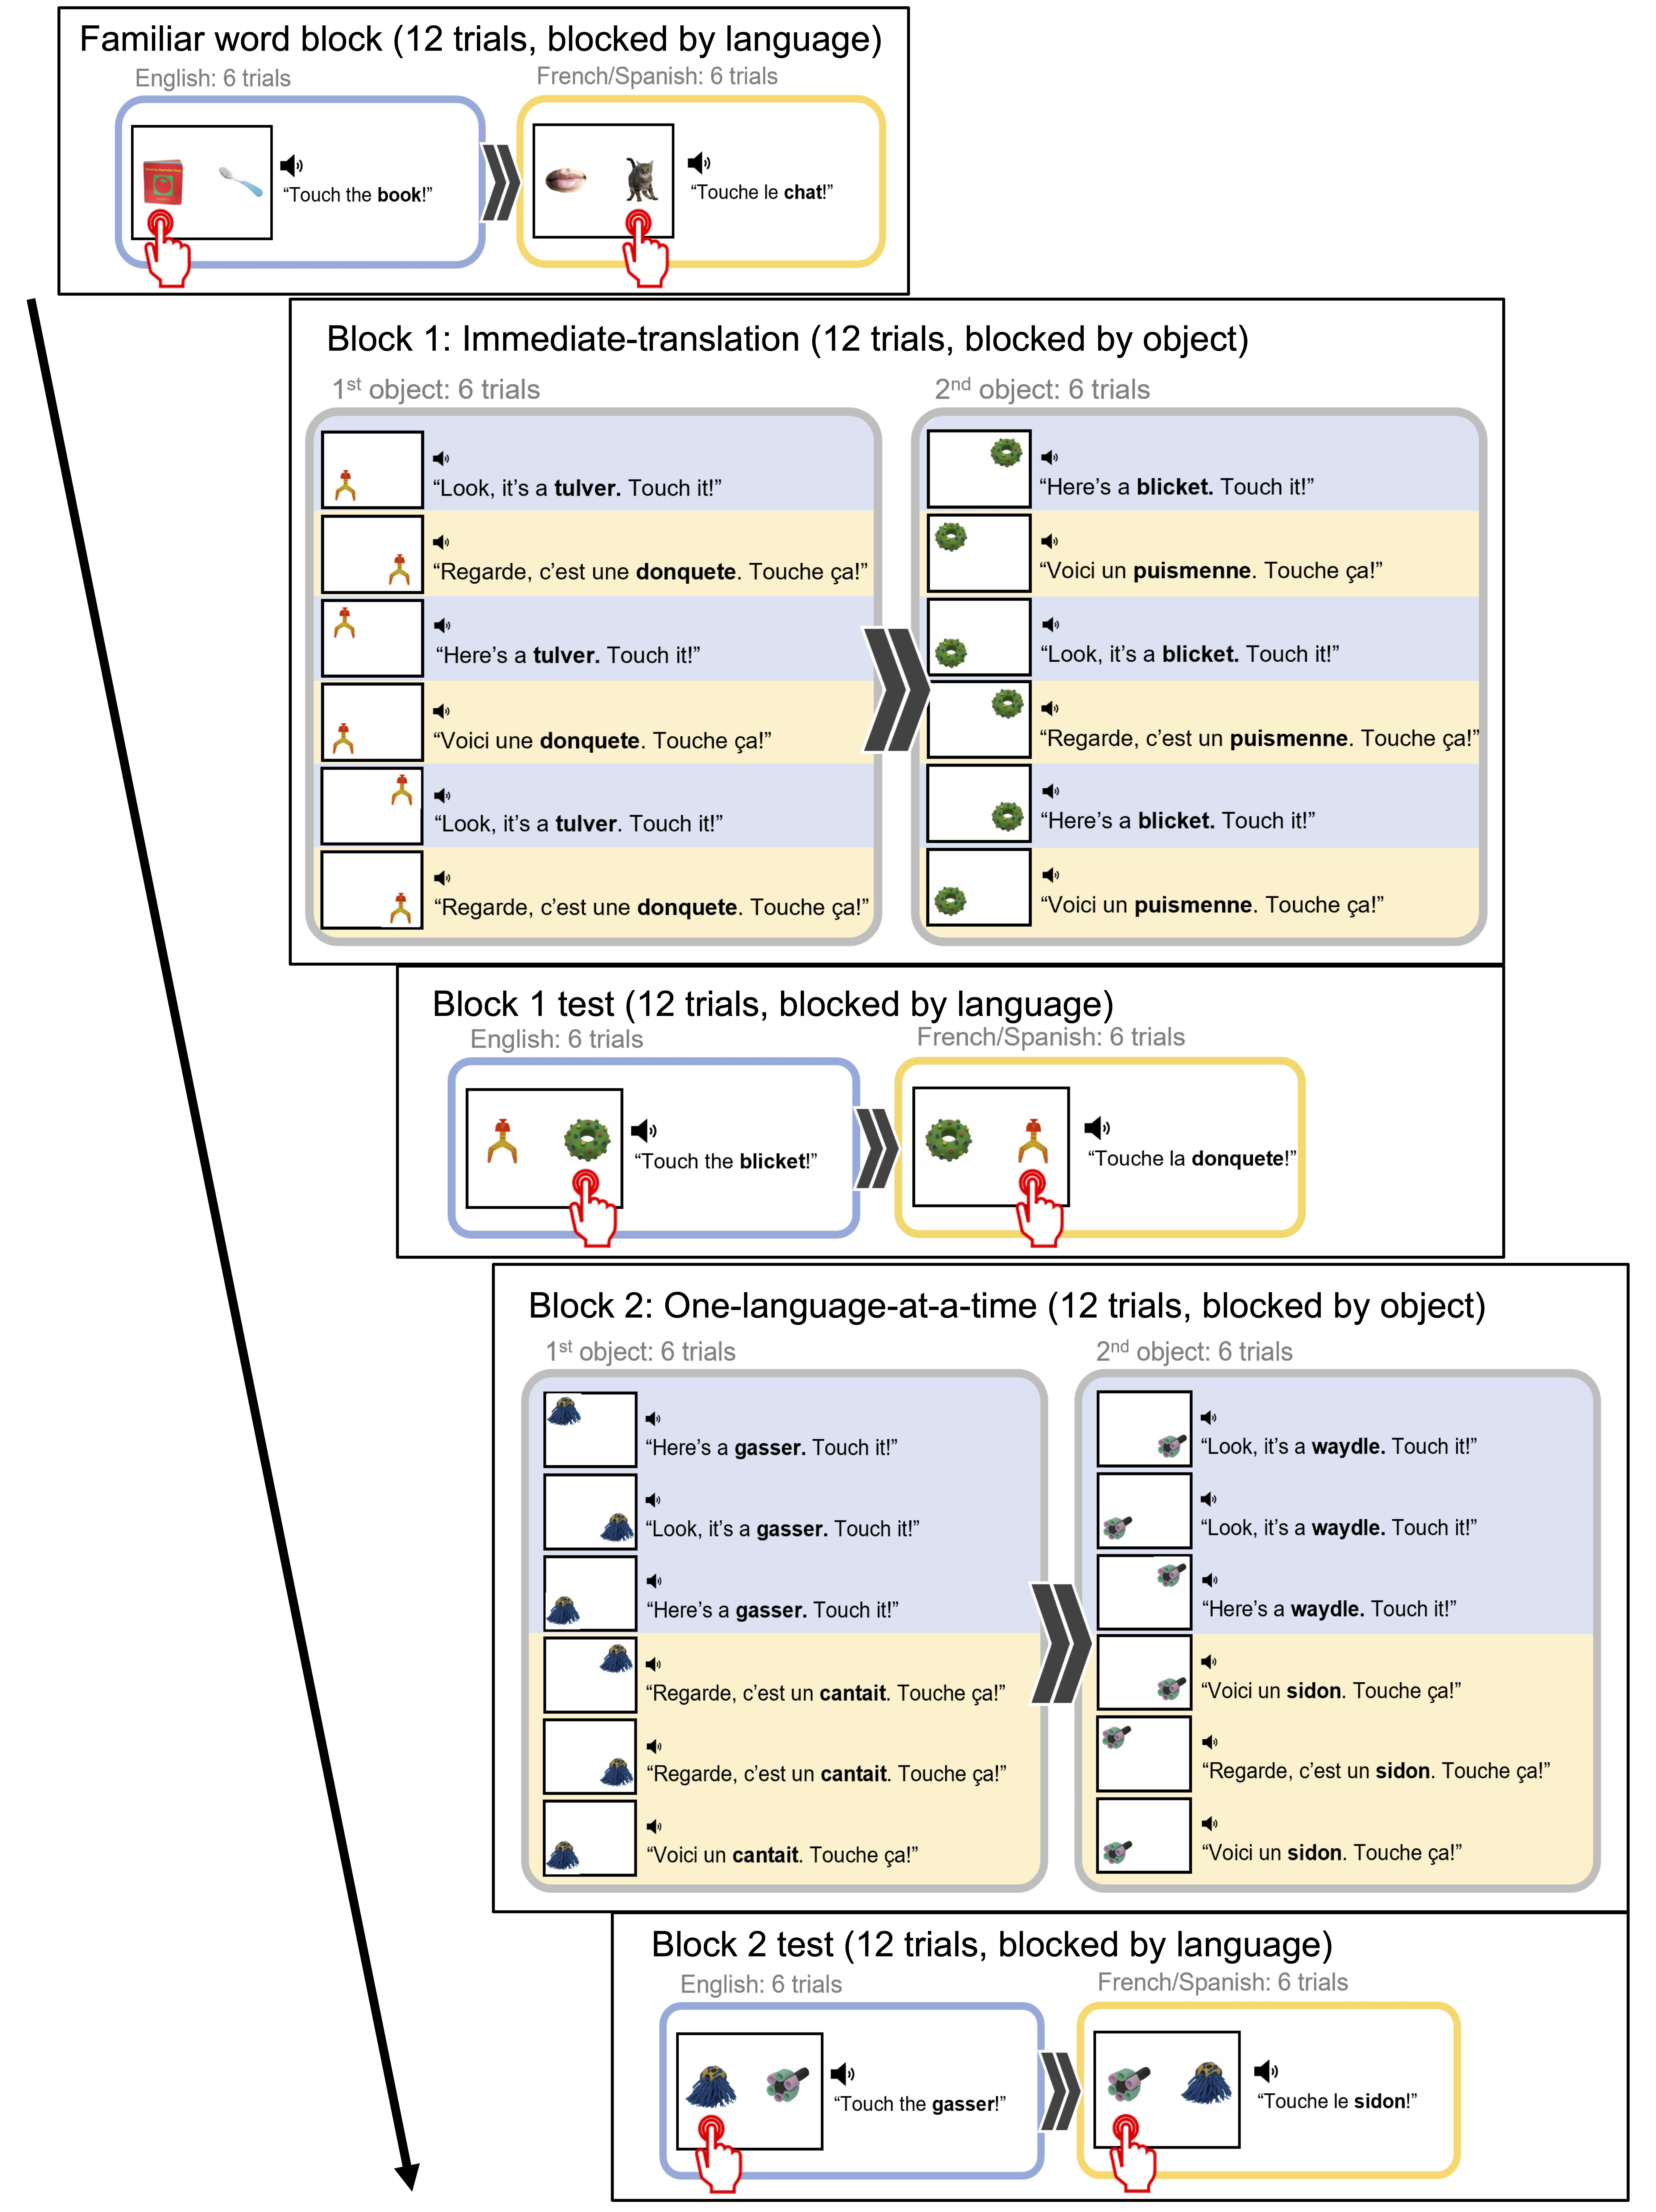
\includegraphics[width=0.9\linewidth]{/Users/racheltsui/Documents/GitHub/Bilingual-Families-Project_TabletSwitch/analysis/paper/figure/figure2} 

}

\caption{Illustration of the task procedure, with blue boxes representing trials in English and yellow boxes representing trials in French or Spanish. Orders of condition and language were counterbalanced across participants.   }\label{fig:Figure2}
\end{figure}

To begin the task, children were greeted by an owl character who switched between the two languages (i.e., between English and French in Montreal or between English and Spanish in New Jersey) to orient children to a bilingual language mode. There were three blocks in the forced-choice word-learning task: \emph{familiar word block, block 1 of learning and test phases, block 2 of learning and test phases.}

In the \emph{familiar word block}, a total of 12 trials were administered to familiarize children with the testing procedure. Common nouns served as the target words to test children's language proficiency in English and French or English and Spanish: \emph{book, doggy, kitty, foot, cookie, nose, key, mouth, hand, chair, spoon, doll}\footnote{The corresponding French words were: \emph{livre, chien, chat, pied, biscuit, nez, clé, bouche, main, chaise, cuillère, poupée}; and the corresponding Spanish words were: \emph{libro, perro, gato, pie, galleta, naríz, llave, boca, mano, silla, cuchara, muñeca.}}. The 12 trials were blocked by language with half of the trials in English and half in French/Spanish, and the nouns tested differed across the two languages such that no translation equivalents were tested within children. Two pictures appeared side by side on the screen in silence for 200ms before children were prompted to touch the picture that corresponded to a target word (e.g., ``Touch the \emph{book}!''). If no response was made after 5000ms following the test sentence offset, the test sentences repeated. If the child failed to make a response within 10000ms after the offset of the initial test sentence, the experiment automatically proceeded to the next trial. There was a 300ms blank screen with a chime sound in between trials. Presentation of familiar words was pseudo-randomized within blocks to ensure an equal number of touches to each side of the screen.

The \emph{learning} and \emph{test} phase formed a block, and children were tested in two within-subjects conditions presented in two separate blocks: the \emph{immediate-translation} condition and the \emph{one-language-at-a-time} condition. In total, there were four test orders created by crossing order of the conditions across blocks, and the order of stimulus' language (English first vs.~French/Spanish first).

In the \emph{learning phase}, children were exposed to two novel label-object pairings six times each across a total of 12 trials. The presentation was blocked by object such that children saw one of the two novel label-object pairings in the first six trials and the other novel label-object pairing in the remaining six trials, with the order of target objects randomized across participants. Each trial presented a novel object appearing alone at one of the four corners of the screen (i.e., top right, top left, bottom right, bottom left), with the position pseudo-randomized to ensure an equal number of appearances at each corner. Similar to the procedure in the familiar word block, audio stimuli played 200ms after the trial onset and children were asked to touch the novel object with the mention of the novel label.

In the \emph{immediate-translation} condition, English trials and French/Spanish trials were interleaved, such that adjacent trials provided an immediate translation; whereas in the \emph{one-language-at-a-time} condition, labels for a particular object were blocked by language. For example, in the \emph{immediate-translation} condition, one child might hear the English label \emph{``tulver''} on trials 1/3/5, and the French label \emph{``donquete''} on trials 2/4/6, where both labels referred to the same object. For the same child in the \emph{one-language-at-a-time} condition, they might hear the English label \emph{``gasser''} on trials 7-9, and the French label \emph{``cantait''} on trials 10-12, again both referring to the same object.

Responses were allowed while the audio stimulus played, but the trial ended only after the entire stimulus was played to ensure that children heard the complete novel label. If no response was made after 5000ms following the audio offset, a whistle sound played to capture children's attention again. The task skipped to the next trial if no response was made within 10000ms upon the initial audio offset; these trials were later excluded in the analysis (see the results section below). A blank screen with a 300ms chime was played as an inter-trial interval.

The \emph{test phase} consisted of a total 12 trials blocked by language with half of trials in English and half in French or Spanish. Each novel label-object pairing was tested three times in each language. The trial structure was the same as in the \emph{familiar word block}. The presentation of the target objects was pseudo-randomized to ensure an equal number of appearances on each side of the screen, and children did not receive feedback about their performance at test.

Upon the completion of Block 1, children proceeded to Block 2 which followed the same procedure as in Block 1 (e.g., learning phase followed by test phase). Finally, we verified with caregivers whether they noticed any task or technical issues.

\hypertarget{results}{%
\section{Results}\label{results}}

Our analysis plan was preregistered at \url{https://osf.io/ad7fz}. Mixed-effects analyses were performed in the R statistical language (Version 4.1.3; R Core Team. 2020) using the lme4 package (Bates et al., 2015), and p-values of the models were calculated using the lmerTest package (Kuznetsova et al., 2017). In the following models, categorical variables were contrast coded such that the intercept of a model represents the mean of all data points in the data set. Post-hoc analyses were conducted through pairwise comparisons using the emmeans package (Lenth, 2022). We reported the main analysis on accuracy here in this paper; exploratory analyses are also reported in the supplemental materials at OSF (\url{https://osf.io/8vk3b/}).

\hypertarget{accuracy}{%
\subsection{Accuracy}\label{accuracy}}

Our primary dependent variable in determining bilingual children's word learning was their accuracy in touching the labeled target object on each test trial. A score of 1 was given to a correct response and a score of 0 to an incorrect response. This type of scoring motivated the use of a logistic mixed-effects regression model. There were two predictor variables: (1) condition with two levels of \emph{immediate-translation} vs.~\emph{one-language-at-a-time}; and (2) language community with two levels of French--English vs.~Spanish--English bilinguals\footnote{Our preregistered analysis plan was to include a predictor variable indicating whether the target word tested was in the children's dominant or non-dominant language. As eight of the 31 French--English children and six of the 22 Spanish--English children were reported to have equal proficiency in both languages, in the end we did not include dominant language as a fixed effect in our models.}.

Following our preregistration, 15 familiar word trials and 70 test trials were excluded where a child did not make any response, resulting in a total of 621 valid familiar word trials and 1195 valid test trials included in the analysis; no more than 10 trials (28\%) were excluded for any individual child. Separate analyses were run for the \emph{familiar word block} and the \emph{test blocks}.

\hypertarget{familiar-word-block}{%
\subsubsection{Familiar word block}\label{familiar-word-block}}

French--English bilingual children showed a mean accuracy of 0.98 on the familiar English-word trials (\(SD\) = 0.06; range = 0.83 -- 1) and 0.97 on the familiar French-word trials (\(SD\) = 0.07; range = 0.8 -- 1). Meanwhile, Spanish--English bilingual children showed a mean accuracy of 0.99 in the familiar English-word trials (\(SD\) = 0.04; range = 0.83 -- 1) and 0.92 in the familiar Spanish-word trials (\(SD\) = 0.19; range = 0.4 -- 1).

We ran a logistic mixed-effects model with proportion of accuracy in the familiar word block as the dependent variable, language (English vs.~French/Spanish) and language community (French--English vs.~Spanish--English) as fixed effects\footnote{We had preregistered that we would enter condition as a fixed effect, which is nonsensical as there was no condition manipulation in the familiar block; language of the familiar nouns tested (i.e., English vs.~French/Spanish) were entered instead.}, and random intercepts of participants and stimulus item:

accuracy \textasciitilde{} language * lang\_community + (1\textbar participant) + (1\textbar item)

\noindent The coefficient estimates from this model are shown in Table 1. While the effect of language community was not significant, the effect of language was significant and the interaction between language and language community approached the significance level of .05. However, post-hoc pairwise comparisons indicated that neither the French--English children nor the Spanish--English children differ significantly in their accuracy across trials in the two languages (French--English: estimate = 0.00, \(SE\) = 0.01, \(z\) = 0.36, \(p\) = 0.72; Spanish--English: estimate = 0.03, \(SE\) = 0.02, \(z\) = 1.24, \(p\) = 0.22). Therefore, both groups of bilingual children generally performed at ceiling and performed similarly in the familiar word block.

\hypertarget{test-blocks}{%
\subsubsection{Test blocks}\label{test-blocks}}

On average, French--English bilingual children showed a mean accuracy of 0.7 in the \emph{immediate-translation} condition (\(SD\) = 0.26; range = 0 -- 1) and 0.7 in the \emph{one-language-at-a-time} condition (\(SD\) = 0.28; range = 0 -- 1). On the other hand, Spanish--English bilingual children showed a mean accuracy of 0.76 in the \emph{immediate-translation} condition (\(SD\) = 0.2; range = 0.25 -- 1) and 0.73 in the \emph{one-language-at-a-time} condition (\(SD\) = 0.24; range = 0.33 -- 1).

To address our research question about whether different language switching patterns would impact bilingual children's word learning, we ran a logistic mixed-effects model on the proportion of accuracy in the test trials, with condition and language community as fixed effects, as well as a random slope of condition by participants and a random intercept of item:

accuracy \textasciitilde{} condition * lang\_community + (1 + condition\textbar participant) + (1\textbar item)

\noindent The coefficient estimates from this model are shown in Table 1, and Figure 3 visualizes this model. There were no significant effects or interactions. Furthermore, separate one-sample t-tests were run on the proportion of accuracy in each condition per community\footnote{The French--English bilinguals performed significantly above the at-chance level in the \emph{immediate-translation} condition (\(t\)(30) = 4.24, \(p < .001\)) and the \emph{one-language-at-a-time} condition (\(t\)(30) = 4.08, \(p < .001\)). Likewise, the Spanish--English bilinguals performed significantly above the at-chance level in the \emph{immediate-translation} condition (\(t\)(21) = 5.98, \(p < .001\)) and the \emph{one-language-at-a-time} condition (\(t\)(21) = 4.52, \(p < .001\)).}. These analyses confirmed that children from both communities learned the novel words in each condition significantly above the at-chance level of 0.50 (all \(p\)s \textless{} .001). In other words, bilingual children in both communities showed strong evidence of word learning, with no difference across the \emph{immediate-translation} and \emph{one-language-at-a-time} conditions.

\begin{table}

\caption{\label{tab:unnamed-chunk-8}Table 1. Coefficient estimates from the logistic mixed-effects models predicting accuracy in the familiar word block and the test blocks.}
\centering
\fontsize{12}{14}\selectfont
\begin{tabular}[t]{lcccc}
\toprule
  & Estimate & SE & z & p\\
\midrule
\addlinespace[0.3em]
\multicolumn{5}{l}{\textbf{Familiar word block}}\\
\hspace{1em}Intercept & 4.740 & 0.762 & 6.220 & <.001\\
\hspace{1em}language & -1.490 & 0.686 & -2.170 & <.05\\
\hspace{1em}lang\_community & 0.133 & 0.858 & 0.155 & 0.877\\
\hspace{1em}language * lang\_community & -2.430 & 1.320 & -1.840 & 0.066\\
\addlinespace[0.3em]
\multicolumn{5}{l}{\textbf{Test blocks}}\\
\hspace{1em}Intercept & 1.200 & 0.220 & 5.600 & <.001\\
\hspace{1em}condition & 0.100 & 0.310 & 0.330 & 0.74\\
\hspace{1em}lang\_community & 0.230 & 0.390 & 0.610 & 0.54\\
\hspace{1em}condition * lang\_community & -0.010 & 0.600 & -0.020 & 0.98\\
\bottomrule
\end{tabular}
\end{table}

\begin{figure}

{\centering 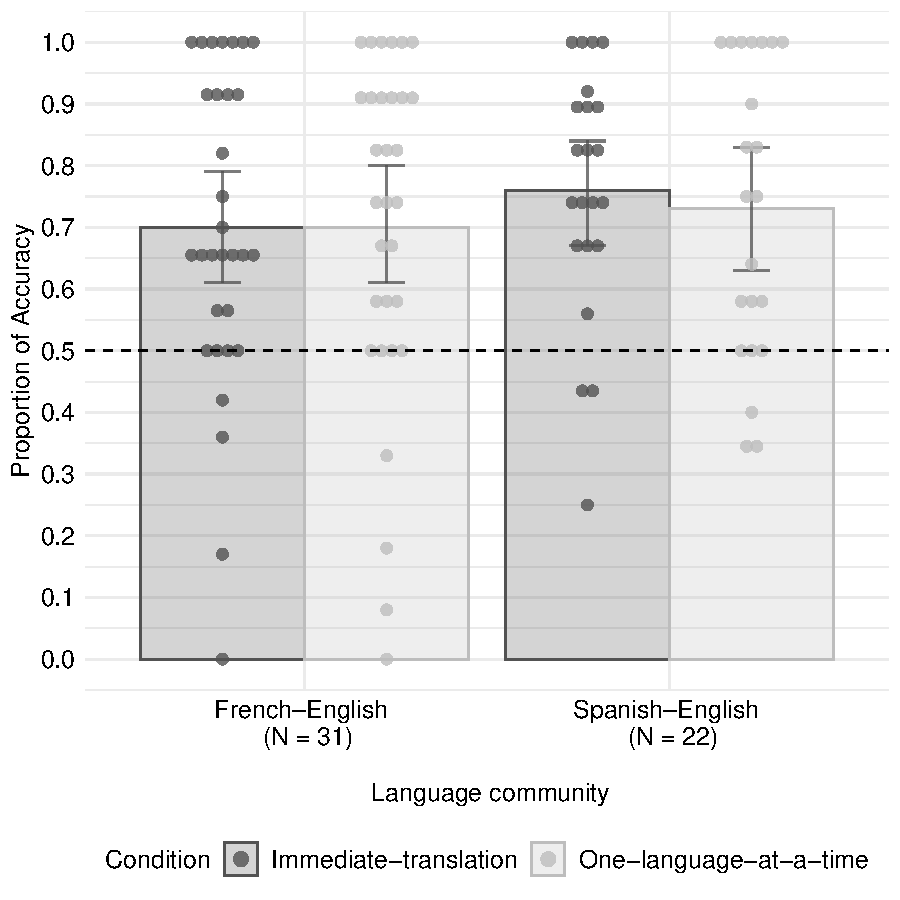
\includegraphics[width=0.6\linewidth]{TabletSwitch_paper_files/figure-latex/Figure3-1} 

}

\caption{Average proportion of accuracy by condition and language community in the test blocks. Dots plot the data from each individual participant. Error bars indicate 95\% confidence intervals, and the black dashed line represents the at-chance accuracy level of 0.50.}\label{fig:Figure3}
\end{figure}

\hypertarget{discussion}{%
\section{Discussion}\label{discussion}}

To better understand whether the dynamics of language switching affect bilingual children's word learning, the current study compared whether children learn novel cross-language words differently if they hear a translation immediately after being named in one language or if they hear the translation more separated in time. Using an online tablet word-learning task, 3- to 5-year-old French--English and Spanish--English bilingual children showed successful learning when they encountered either type of language switch, a pattern which was similar across the two bilingual communities. Therefore, our results indicate that variation in language switching patterns does not affect word learning. Overall, our findings highlight that different patterns of language switching provide equal learning opportunities for vocabulary development among children growing up in different bilingual communities.

Children's successful performance in this experiment suggests that their word learning is supported in environments that include regular language switching. Contrary to studies reporting that language switching is associated with less successful word learning for bilingual children (Byers-Heinlein, 2013; Carbajal \& Peperkamp, 2020), our findings are in line with studies showing that language switching does not hinder but could support language learning (Bail, 2015; De Houwer, 2007; Kremin et al., 2021b; Orena \& Pola, 2019). Our study was novel in using an online tablet touchscreen task, and our findings are congruent with results using bilingual book reading methods. For example, Brouillard et al.~(2022) showed that 5-year-old French--English bilingual children were able to learn words in both languages and were not affected by whether languages were interleaved or blocked in the books. Similar results have also been reported in another study with Spanish--English bilingual children (Read et al., 2021), although this study tested word learning in bilingual children's non-dominant language only. Overall, current evidence confirms that bilingual children effectively learn cross-language words in each of their two languages across different patterns of language switching.

Moreover, children from both bilingual communities were equally able to learn words under different switching patterns. While previous studies have reported that bilingual caregivers inevitably show different behaviors when switching between their languages (Bail et al., 2015; Kremin et al., 2021a), our results revealed that bilingual children from different communities do not necessarily learn words differently under different language switching patterns. The lack of language community differences suggests that children's ability to learn words in different switching contexts is unaffected by the patterns of switching they typically hear, a possibility that will need to be tested in future studies with children from a wider variety of communities.

Our experiment used a highly-controlled experimental design, which gave children equal opportunities to learn words in two languages, with equal exposure to each word as well as equal information presented in both languages and across both conditions. However, this may not reflect caregivers' everyday behaviors. While bilingual caregivers often switch languages to enhance their children's understanding of translation equivalents in both languages (Kremin et al., 2021a), sometimes they may also switch languages when having a hard time retrieving a word from the other language in the moment (Heredia \& Altarriba, 2001). Moreover, bilingual parents may generally use one of their languages more often than the other (Orena et al., 2020). Therefore, bilingual children's exposure to words across their languages is likely to be less systematic than in our study. Previous research has shown that the amount of exposure to a specific language matters, with bilingual children often learning more words in the language to which they hear a greater amount of exposure (David \& Wei, 2008; Hoff et al., 2012; Marchman et al., 2017; Pearson et al., 1993). It is possible that different frequencies of exposure to each language may interact with learning across different contexts of language switching. Future studies may consider using a less-balanced experimental design to test whether different language switching patterns (e.g., many switches from Spanish to English, but not vice-versa) would still allow bilingual children to learn cross-language words equally.

Our study was also limited to testing children's learning from inter-sentential language switching, as in both of our conditions language switches happened across sentence boundaries where all words within a single sentence were in the same language. However, caregivers may also switch languages within a single sentence, where words from the two languages are embedded within the same sentence (e.g., a French--English bilingual caregiver may say ``Look, it's a \emph{chien}!'' to their child when they see a dog on the street). Previous research has reported that bilingual children may have difficulty processing speech that contains a within-sentence language switch, but have relatively little difficulty processing speech that contains a between-sentence switch (Byers-Heinlein et al., 2017; Morini \& Newman, 2019; Potter et al., 2019). It is plausible that the language switching patterns we explored in this study could be less challenging for children to process than other types of switching. Although bilingual caregivers tend to switch more often between sentences than within sentences (Bail et al., 2015; Kremin et al., 2021a), it is still important for future studies to explore whether bilingual children's word learning would be impacted by differences in the syntactic location of when language switches occur.

\hypertarget{conclusion}{%
\section{Conclusion}\label{conclusion}}

Overall, our findings provide new evidence that may ease caregivers' concerns about how to best raise their bilingual children's language development. Many bilingual caregivers wonder how they should introduce words in each language to their child. Our findings suggest that there are multiple ways to do so effectively, as differences in the timing of language switches do not necessarily result in different word learning outcomes. Whether bilingual children hear a translation immediately or more separated in time, either type of language switching supports and provides meaningful opportunities for word learning. Future studies that incorporate different patterns of exposure to novel words would be important to fully understand the effect of language switching patterns in early bilingual vocabulary development. Nonetheless, the main take home message from our study for bilingual caregivers is that, rather than following a strict language switching pattern, it is reasonable to interact with their children in a way that makes them comfortable, while at the same time supporting children by offering meaningful experience with each of their languages.

\newpage

\hypertarget{references}{%
\section{References}\label{references}}

\begingroup
\setlength{\parindent}{-0.5in}

\hypertarget{refs}{}
\begin{CSLReferences}{1}{0}
\leavevmode\vadjust pre{\hypertarget{ref-Ahooja_et_al_2022}{}}%
Ahooja, A., Brouillard, M., Quirk, E., Ballinger, S., Polka, L., Byers-Heinlein, K., \& Kircher, R. (2022). Family language policy among {Québec}-based parents raising multilingual infants and toddlers: A study of resources as a form of language management. \emph{Journal of Multilingual and Multicultural Development}, 1--20. \url{https://doi.org/doi.org/10.1080/01434632.2022.2050918}

\leavevmode\vadjust pre{\hypertarget{ref-Bail_etal_2015}{}}%
Bail, A., Morini, G., \& Newman, R. S. (2015). Look at the gato! Code-switching in speech to toddlers. \emph{Journal of Child Language}, \emph{42}(5), 1073--1101. \url{https://doi.org/10.1017/S0305000914000695}

\leavevmode\vadjust pre{\hypertarget{ref-Bates_etal_2015}{}}%
Bates, M., D., \& Walker, S. (2015). Fitting linear mixed-effects models using lme4. \emph{Journal of Statistical Software}, \emph{67}(1), 1--48. \url{https://doi.org/10.18637/jss.v067.i01}

\leavevmode\vadjust pre{\hypertarget{ref-Benitez_etal_2022}{}}%
Benitez, V. L., Castellana, M., \& Potter, C. E. (2022). How many palabras? Codeswitching and lexical diversity in {Spanish-English} picture books. \emph{Languages}, \emph{7}, 69. \url{https://doi.org/10.3390/languages7010069}

\leavevmode\vadjust pre{\hypertarget{ref-Brouillard_etal_2022}{}}%
Brouillard, M., Dubé, D., \& Byers-Heinlein, K. (2022). Reading to bilingual preschoolers: An experimental study of two book formats. \emph{Infant and Child Development}, e2294. \url{https://doi.org/10.1002/icd.2294}

\leavevmode\vadjust pre{\hypertarget{ref-Buoy_Nicoladis_2018}{}}%
Buoy, T., \& Nicoladis, E. (2018). The considerateness of codeswitching: A comparison of two groups of {Canadian French-English} bilinguals. \emph{Journal of Intercultural Communication Research}, \emph{47}(4), 361--373. \url{https://doi.org/10.1080/17475759.2018.1462241}

\leavevmode\vadjust pre{\hypertarget{ref-Byers_2013}{}}%
Byers-Heinlein, K. (2013). Parental language mixing: Its measurement and the relation of mixed input to young bilingual children's vocabulary size. \emph{Bilingualism: Language and Cognition}, \emph{16}(1), 32--48. \url{https://doi.org/10.1017/S1366728912000120}

\leavevmode\vadjust pre{\hypertarget{ref-Byers_etal_2017}{}}%
Byers-Heinlein, K., Morin-Lessard, E., \& Lew-Williams, C. (2017). Bilingual infants control their languages as they listen. \emph{Proceedings of the National Academy of Sciences}, \emph{114}(34), 9032--9037. \url{https://doi.org/10.1073/pnas.1703220114}

\leavevmode\vadjust pre{\hypertarget{ref-Carbajal_Peperkamp_2020}{}}%
Carbajal, M. J., \& Peperkamp, S. (2020). Dual language input and the impact of language separation on early lexical development. \emph{Infancy}, \emph{25}(1), 22--45. \url{https://doi.org/10.1111/infa.12315}

\leavevmode\vadjust pre{\hypertarget{ref-David_Wei_2008}{}}%
David, A., \& Wei, L. (2008). Individual differences in the lexical development of {F}rench--{E}nglish bilingual children. \emph{International Journal of Bilingual Education and Bilingualism}, \emph{11}(5), 598--618. \url{https://doi.org/10.1080/13670050802149200}

\leavevmode\vadjust pre{\hypertarget{ref-DeHouwer_2007}{}}%
De Houwer, A. (2007). Parental language input patterns and children's bilingual use. \emph{Applied Psycholinguistic}, \emph{28}(3), 441--424. \url{https://doi.org/10.1017/S0142716407070221}

\leavevmode\vadjust pre{\hypertarget{ref-Fennell_Lew_2017}{}}%
Fennell, C., \& Lew-Williams, C. (2017). Early bilingual word learning. In G. Westermann \& N. Mani (Eds.), \emph{Early word learning} (pp. 110--122). Routledge.

\leavevmode\vadjust pre{\hypertarget{ref-Gardner_etal_2005}{}}%
Gardner-Chloros, P., McEntee-Atalianis, L., \& Finnis, K. (2005). Language attitudes and use in a transplanted setting: {Greek Cypriots} in {London}. \emph{International Journal of Multilingualism}, \emph{2}(1), 52--80. \url{https://doi.org/10.1080/17501220508668376}

\leavevmode\vadjust pre{\hypertarget{ref-Grammont_1902}{}}%
Grammont, M. (1902). \emph{Observations sur le langage des enfants}. Melanges Meillet.

\leavevmode\vadjust pre{\hypertarget{ref-Heredia_Altarriba_2001}{}}%
Heredia, R. R., \& Altarriba, J. (2001). Bilingual language mixing: Why do bilinguals code-switch? \emph{Current Directions in Psychological Science}, \emph{10}(5), 164--168. \url{https://doi.org/10.1111/1467-8721.00140}

\leavevmode\vadjust pre{\hypertarget{ref-Kircher_etal_2022}{}}%
Kircher, R., Quirk, E., Brouillard, M., Ahooja, A., Ballinger, S., Polka, L., \& Byers-Heinlein, K. (2022). Quebec-based parents' attitudes towards childhood multilingualism: Evaluative dimensions and potential predictors. \emph{Journal of Language and Social Psychology}, \emph{41}(5), 527--552. \url{https://doi.org/10.1177/0261927X22107885}

\leavevmode\vadjust pre{\hypertarget{ref-Kosie_etal_prep}{}}%
Kosie, J. E., Tsui, R. K.-Y., Martinez, T., Sander, A., Fibla, L., Potter, C., Byers-Heinlein, K., \& Lew-Williams, C. (in preparation). \emph{Cross-community differences in bilingual infants' experience with language switching}.

\leavevmode\vadjust pre{\hypertarget{ref-Kremin_etal_2021a}{}}%
Kremin, L. V., Alves, J., Orena, A. J., Polka, L., \& Byers-Heinlein, K. (2021a). Code-switching in parents' everyday speech to bilingual infants. \emph{Journal of Child Language}, \emph{First View}, 1--27. \url{https://doi.org/10.1017/S0305000921000118}

\leavevmode\vadjust pre{\hypertarget{ref-Kremin_etal_2021b}{}}%
Kremin, L. V., Jardak, A., Lew-Williams, C., \& Byers-Heinlein, K. (2021b). \emph{Bilingual children's comprehension of code-switching at an uninformative adjective} {[}PsyArxiv Preprint{]}. \url{https://doi.org/10.31234/osf.io/akz96}

\leavevmode\vadjust pre{\hypertarget{ref-Kuznetsova_etal_2017}{}}%
Kuznetsova, A., Brockhoff, P. B., \& Christensen, R. H. B. (2017). lmerTest package: Tests in linear mixed effects models. \emph{Journal of Statistical Software}, \emph{82}(13), 1--26. \url{https://doi.org/10.18637/jss.v082.i13}

\leavevmode\vadjust pre{\hypertarget{ref-Lenth_2022}{}}%
Lenth, R. V. (2022). \emph{Emmeans: Estimated marginal means, aka least-squares means} (Version 1.7.2) {[}Computer software{]}. \url{https://CRAN.R-project.org/package=emmeans}

\leavevmode\vadjust pre{\hypertarget{ref-migration_policy_institute_2021}{}}%
Migration Policy Institute. (2021). \emph{Tabulation of data from the u.s. Census bureau's pooled 2015-2019 american community survey on u.s. Young children (ages 0 to 8) by dual language learner status: National and state sociodemographic and family profiles}. National Center on Immigrant Integration Policy. \url{https://www.migrationpolicy.org/programs/data-hub/charts/us-state-profiles-young-dlls}

\leavevmode\vadjust pre{\hypertarget{ref-Montes_2000}{}}%
Montes-Alcalá, C. (2000). Attitudes towards oral and written codeswitching in spanish--english bilingual youths. In A. Roca (Ed.), \emph{Research on spanish in the u.s.} (pp. 218--227). Cascadilla.

\leavevmode\vadjust pre{\hypertarget{ref-Morini_Newman_2019}{}}%
Morini, G., \& Newman, R. S. (2019). Dónde está la ball? Examining the effect of code switching on bilingual children's word recognition. \emph{Journal of Child Language}, \emph{46}(6), 1238--1248. \url{https://doi.org/10.1017/S0305000919000400}

\leavevmode\vadjust pre{\hypertarget{ref-Myers-Scotton_2017}{}}%
Myers-Scotton, C. (n.d.). Code-switching. In F. Coulmas (Ed.), \emph{The handbook of sociolinguistics} (pp. 217--237). Blackwell Publishing Ltd. \url{https://doi.org/10.1002/9781405166256.ch13}

\leavevmode\vadjust pre{\hypertarget{ref-Orena_Polka_2019}{}}%
Orena, A. J., \& Polka, L. (2019). Monolingual and bilingual infants' word segmentation abilities in an inter-mixed dual-language task. \emph{Infancy}, \emph{24}(5), 718--737. \url{https://doi.org/10.1111/infa.12296}

\leavevmode\vadjust pre{\hypertarget{ref-Pearson_etal_1993}{}}%
Pearson, B. Z., Fernández, S. C., \& Oller, D. K. (1993). Lexical development in bilingual infants and toddlers: Comparison to monolingual norms. \emph{Language Learning}, \emph{43}(1), 93--120. \url{https://doi.org/10.1111/j.1467-1770.1993.tb00174.x}

\leavevmode\vadjust pre{\hypertarget{ref-Place_Hoff_2011}{}}%
Place, S., \& Hoff, E. (2011). Properties of dual language exposure that influence 2-year-olds' bilingual proficiency. \emph{Child Development}, \emph{82}(6), 1834--1849. \url{https://doi.org/10.1111/j.1467-8624.2011.01660.x}

\leavevmode\vadjust pre{\hypertarget{ref-Poplack_1980}{}}%
Poplack, S. (1980). Sometimes {I'll} start a sentence in {Spanish} y termino en espanol: Toward a typology of code-switching. \emph{Linguistics}, \emph{18}, 581--618. \url{https://doi.org/10.1515/ling.1980.18.7-8.581}

\leavevmode\vadjust pre{\hypertarget{ref-Poplack_1988}{}}%
Poplack, S. (1988). Contrasting patterns of code-switching in two communities. \emph{Codeswitching: Anthropological and Sociolinguistic Perspectives}, \emph{48}, 215--244. \url{https://doi.org/10.1515/9783110849615}

\leavevmode\vadjust pre{\hypertarget{ref-Potter_etal_2019}{}}%
Potter, C. E., Fourakis, E., Morin-Lessard, E., Byers-Heinlein, K., \& Lew‐Williams, C. (2019). Bilingual toddlers' comprehension of mixed sentences is asymmetrical across their two languages. \emph{Developmental Science}, \emph{22}(4), e12794. \url{https://doi.org/10.1111/desc.12794}

\leavevmode\vadjust pre{\hypertarget{ref-Quirk_etal_2022}{}}%
Quirk, E., Brouillard, M., Ahooja, A., Ballinger, S., Polka, L., Byers-Heinlein, K., \& Kircher, R. (2022). \emph{Quebec-based parents' concerns regarding their children's multilingual development} {[}PsyArxiv Preprint{]}. \url{https://doi.org/10.31234/osf.io/583ge}

\leavevmode\vadjust pre{\hypertarget{ref-R_2019}{}}%
R Core Team. (2020). \emph{R: A language and environment for statistical computing} (Version 4.1.3) {[}Computer software{]}. R Foundation for Statistical Computing. \url{https://www.R-project.org/}

\leavevmode\vadjust pre{\hypertarget{ref-Read_etal_2021}{}}%
Read, K., Contreras, P. D., Rodriguez, B., \& Jara, J. (2021). ¿Read conmigo?: The effect of code-switching storybooks on dual-language learners' retention of new vocabulary. \emph{Early Education and Development}, \emph{32}(4), 516--533. \url{https://doi.org/10.1080/10409289.2020.1780090}

\leavevmode\vadjust pre{\hypertarget{ref-Ronjat_1913}{}}%
Ronjat, J. (1913). \emph{Le développement du langage observé chez un enfant bilingue}. Champion.

\leavevmode\vadjust pre{\hypertarget{ref-Schott_etal_2022}{}}%
Schott, E., Kremin, L. V., \& Byers-Heinlein, K. (2022). The youngest bilingual {Canadians}: Insights from the 2016 census regarding children aged 0--9 years. \emph{Canadian Public Policy}, \emph{48}(2), 254--266. \url{https://doi.org/10.3138/cpp.2021-064}

\leavevmode\vadjust pre{\hypertarget{ref-Thibeault_Matheson_2020}{}}%
Thibeault, J., \& Matheson, I. A. (2020). The cross-linguistic reading strategies used by elementary students in {French} immersion as they engage with dual-language children's books. \emph{Canadian Modern Language Review}, \emph{76}(4), 375--394. \url{https://doi.org/10.3138/cmlr-2019-0071}

\leavevmode\vadjust pre{\hypertarget{ref-Toribio_2022}{}}%
Toribio, A. J. (2022). {Spanish-English} code-switching among {US Latinos}. \emph{International Journal of the Sociology of Language}, \emph{158}, 89--119. \url{https://doi.org/10.1515/ijsl.2002.053}

\end{CSLReferences}

\endgroup


\end{document}
